\section{Zielsetzung}
\label{sec:Zielsetzung}
Ziel dieses Versuches ist es die grundlegenden physikalischen Eigenschaften und Begriffe der Ultraschallechographie zu lernen und anzuwenden. 
Dazu wird bei verschiedenen Körpern durch verschiedene Verfahren die Laufzeit gemessen.

\section{Theorie}
\label{sec:Theorie}
Ultraschall besitzt einen Frequenzbereich zwischen $20 \si{\kilo\Hz}$ und $1 \si{\giga\Hz}$, welchen Menschen nicht mehr wahrnehmen können.
Schall im Allgemeinen ist eine longitudinale Welle, welche mit 
\begin{equation*}
    p(x,t) = p_0 + v_0 Z \text{cos}(\omega t - k x)
\end{equation*}
beschrieben werden kann und welche sich aufrgund von Druckschwankungen fortbewegt.
Der Faktor $Z$ ist die akustische Impedanz oder Schallkennwiderstand und wird durch
\begin{equation}
    Z = c \cdot \rho 
    \label{eqn:Impedanz}
\end{equation}
beschrieben, wobei $\rho$ die Dichte des durchstrahlten Materials und $c$ die Schallgeschwindigkeit in diesem Material ist.
Schallwellen zeigen im Allgemeinen das selbe Verhalten wie elektromagnetische Wellen
auf, jedoch ist bei Schallwellen aufgrund der Änderung von Druck und Dichte die
Phasengeschwindigkeit materialabhängig.\\
Aufgrund der Materialabhängigkeit muss bei Schallwellen zwischen gasförmigen bzw. flüssigen Medien und Festkörpern unterschieden werden.
In Gasen und Flüsigkeiten treten lediglich Longitudinalwellen auf, sodass sich für die Schallgeschwindigkeit
\begin{equation}
    c_{Fl} = \sqrt{\frac{1}{\kappa \rho}}
    \label{eqn:cFlüssig}
\end{equation}
ergibt, wobei $\kappa$ die Kompressibilität des Mediums beschreibt.
In Festkörpern treten zusätzlich zu Longitudinalwellen auch Transversalwellen auf. Daraus folgt, dass in Festkörpern die Schallgeschwindigkeit 
grundsätzlich richtungsabhängig ist.
Mit dem Elastizitätmodul $E$ ergibt sich für die Schallgeschwindigkeit
\begin{equation}
    c_{Fe} = \sqrt{\frac{E}{\rho}}.
    \label{eqn:cFest}
\end{equation}
Für Transversalwellen und Longitudinalwellen ist $c_{Fe}$ unterschiedlich.\\
Bei der Betrachtung von Schallwellen in einem Medium geht ein Teil der Energie durch Absorption verloren.
Die Intensität der Welle 
\begin{equation}
    I(x) = I_0 \text{e}^{-\alpha x}
    \label{eqn:Intensi}
\end{equation}
lässt sich als Funktion des Ortes und des Absorptionskoeffizienten $\alpha$ beschreiben. Dabei besitzt Luft einen sehr großen Absorptionskoeffizienten,
weshalb im folgenden Versuch immer ein Kontaktmittel verwendet wird.\\
Während des Experiments werden zwei verschiedene Messmethoden verwendet, wovon eine auf der reflektierten und eine auf der transmittierten Welle basiert.
Der Reflexionskoeffizient 
\begin{equation}
    R = (\frac{Z_1-Z_2}{Z_1+Z_2})^2
\end{equation}
beschreibt das Verhältnis der einfallenden und reflektierten Intensitäten und ist von den akustischen Impedanzen $Z$ abhängig.
Der transmittierte Anteil $T$ lässt sich aus $T = 1 - R$ berechnen.\\
\\
Die Erzeugung von Ultraschall kann auf verschiedene Arten passieren. In diesem Versuch wird nur der piezo-elektrische Effekt betrachtet.
Piezo-elektrische Kristalle können durch Anregung eines äußeren elektrischen Feldes in Schwingungen versetzt werden.
Die Amplitude der entstehenden Welle und die daraus resultierende Energiedichte kann maximiert werden, indem zwischen Anregungsfrequenz und Eigenfrequenz
des Kristalls Resonanz entsteht.
Außerdem können Piezokristalle als Empfänger genutzt werden, weil sie durch Schallwellen angeregt werden.
Dabei ist Quarz der meist verwendete Piezokristall, weil Quarz gleichbleibende physikalische Eigenschaften besitzt.
Jedoch ist der Piezo-Effekt bei Quarzen relativ gering.\\
Mithilfe von Ultraschall können Informationen über der Aufbau eines Stoffes gewonnen werden. Dies wird hauptsächlich mit der Laufzeitmessung gemacht,
welche in diesem Versuch durch zwei Methoden durchgeführt wird. Im Allgemeinen basiert die Messung darauf, dass ein Ultraschallsignal 
losgesendet wird und die Laufzeit auf einer definierten Messstrecke mittels eines Empfängers gemessen wird.\\
\begin{figure}[H]
    \begin{subfigure}{0.48\textwidth}
       \centering
       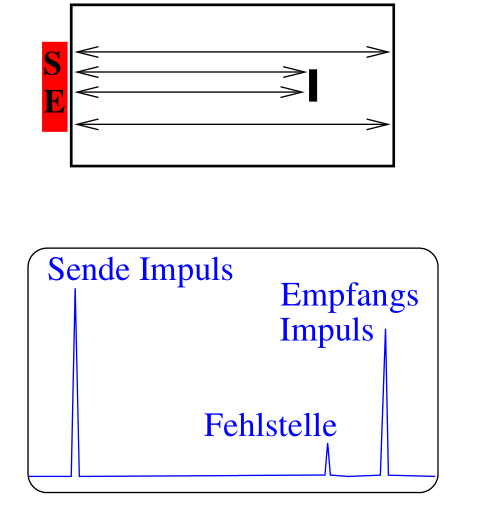
\includegraphics[height=6cm]{build/Impuls_Echo.png}
       \caption{Das Impuls-Echo-Verfahren.}
       \label{fig:ImpulsEcho}
    \end{subfigure}
    \hfill
    \begin{subfigure}{0.48\textwidth}    
        \centering
        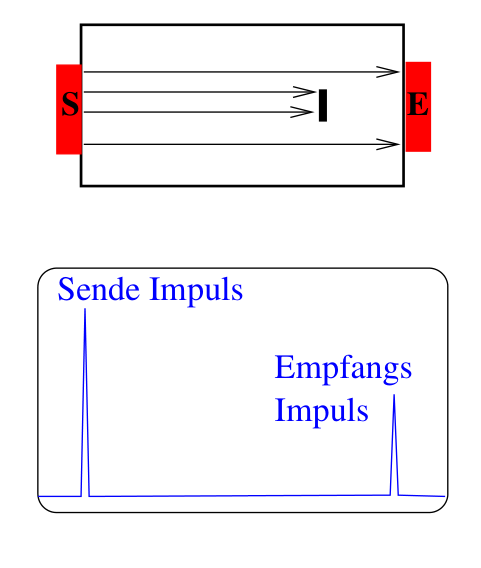
\includegraphics[height=6cm]{build/Durchschall.png}
        \caption{Das Durchschallungs-Verfahren.}
        \label{fig:Durchschallung}
    \end{subfigure}
    \caption{Zwei Messmethoden zur Messung der Laufzeit\cite{VUS1}.}
    \label{fig:Methoden}
\end{figure}
Bei der ersten Methode handelt es sich um das Impuls-Echo-Verfahren (\autoref{fig:ImpulsEcho}). Es wird nur ein Schallkopf verwendet, welcher
sowohl Schallwellen lossendet als auch die reflektierten Signale wahrnimmt.
Mithilfe der Laufzeit kann die Lage der Fehlstelle mit
\begin{equation}
    s = \frac{1}{2} c t
    \label{eqn:Strecke}
\end{equation}
bestimmt werden.\\
Die zweite Methode ist das Durchschallungs-Verfahren, was in \autoref{fig:Durchschallung} schematisch dargestellt ist. 
Dabei werden zwei Ultraschallköpfe benutzt. Einer davon ist der Ultraschallsender und sendet ein Signal, welches auf der anderen Seite von
einem Empfänger aufgenommen wird. Die Intensität wird abgeschwächt, wenn eine Fehlstelle in der Probe vorliegt. Der genaue Ort der 
Fehlstelle kann nicht durch dieses Verfahren bestimmt werden.
